\paragraph{Scopo}
\label{Progettazione_Scopo} \-\\
L'attività di Progettazione consiste nel descrivere una soluzione che sia soddisfacente per gli stakeholder\glossario. È compito dei \textit{Progettisti} svolgere tale attività, definendo l'architettura del prodotto finale, mantenendo chiare e riusabili le componenti, restando nei costi prefissati.\\
L'architettura definita dovrà quindi:
\begin{itemize}
	\item Soddisfare i requisiti definiti nel \textit{Analisi dei Requisiti v2.0.0};
	\item Essere comprensibile e modulare;
	\item Essere robusta riuscendo a gestire situazioni d'errore improvvise.
\end{itemize}

\paragraph{Sviluppo} \-\\
\label{Progettazione_Sviluppo}
Lo sviluppo di \textit{G\&B} avviene seguendo il modello incrementale, spiegato nel dettaglio nel documento \textit{Piano di Progetto v2.0.0} alla sezione §4.\\
La proponente nel capitolato d'appalto pone un singolo vincolo riguardo le tecnologie da utilizzare:
\begin{itemize}
	\item \textit{JavaScrip}t: in particolare nella sua declinazione nota come \textit{ECMAScript 6}\glossario.
\end{itemize}
Tuttavia, ai fini della realizzazione del prodotto finale, il team \texttt{Agents of S.W.E.} ha definito l'uso di ulteriori tecnologie, analizzate di seguito, per scopi diversi:
\begin{itemize} 
	\item \textit{Telegraf}\glossario: è un agente per la raccolta e la rilevazione periodica di metriche\footnote{Metriche d'uso di un elaboratore. Per esempio: percentuale d'uso della CPU, pressione di memoria, etc.} e dati. Si connette ad un database\glossario e vi salva tali dati;
	\item \textit{InfluxDB}\glossario: è un database\glossario per le serie temporali. Verrà utilizzato per il salvataggio dei dati raccolti da \textit{Telegraf};
	\item \textit{JSBayes}\glossario: libreria suggerita dal proponente per la semplice definizione di reti bayesiane; 
	\item \textit{UnBBayes}\glossario: framework e interfaccia grafica per le reti bayesiane. In particolare, verrà utilizzato per la visualizzazione della rete bayesiana in uso all'interno del plug-in, per soddisfare il requisito opzionale 2 esposto all'interno del capitolato d'appalto;
%	\item Docker\glossario\footnote{\url{https://www.docker.com/}}: progetto open-source\glossario che automatizza il deployment\glossario di applicazioni all'interno di contenitori software. In particolare, in Docker Hub\glossario\footnote{\url{https://hub.docker.com/}} sono presenti le immagini utilizzabili mediante container di Telegraf, InfluxDB e Grafana. Pertanto, per agevolare la collaborazione e uniformare l'ambiente di sviluppo, \texttt{Agents Of S.W.E.} utilizzerà Grafana, Telegraf e InfluxDB in appositi container Docker;
	\item \textit{GitLab}\glossario: piattaforma open-source per la gestione di repository \textit{Git}. Il team utilizzerà un repository salvato su tale piattaforma in quanto permette la gestione di una pipeline di CI/CD\glossario, evitando quindi l'uso di altri strumenti. Il processo di CI/CD si configura come rappresentato nell'immagine e viene spiegato nell'appendice \ref{CICD} ;
	\item \textit{NPM}\glossario: manager di pacchetti per \textit{JavaScript}. Verrà analizzato nel dettaglio in §\ref{NPM};
	\item \textit{Jest}\glossario: è un framework per il testing di \textit{JavaScript}. Verrà analizzato nel dettaglio in §\ref{jest};
	\item \textit{Codecov.io}: servizio di code coverage\glossario basato su repository presenti in piattaforme di versionamento quali \textit{GitHub}\glossario e \textit{GitLab}. Ad ogni esecuzione in \textit{GitLab }della pipeline di CI/CD, durante la cui esecuzione vengono generati da \textit{Jest} i report di coverage, \textit{Codecov.io} elabora la copertura del codice;
	\item \textit{jQuery}\glossario: è una libreria \textit{JavaScript} per applicazioni web. Viene utilizzato all'interno del progetto per le  \textit{AJAX}\glossario request.
\end{itemize}

\begin{figure}[H]
	\begin{center}
		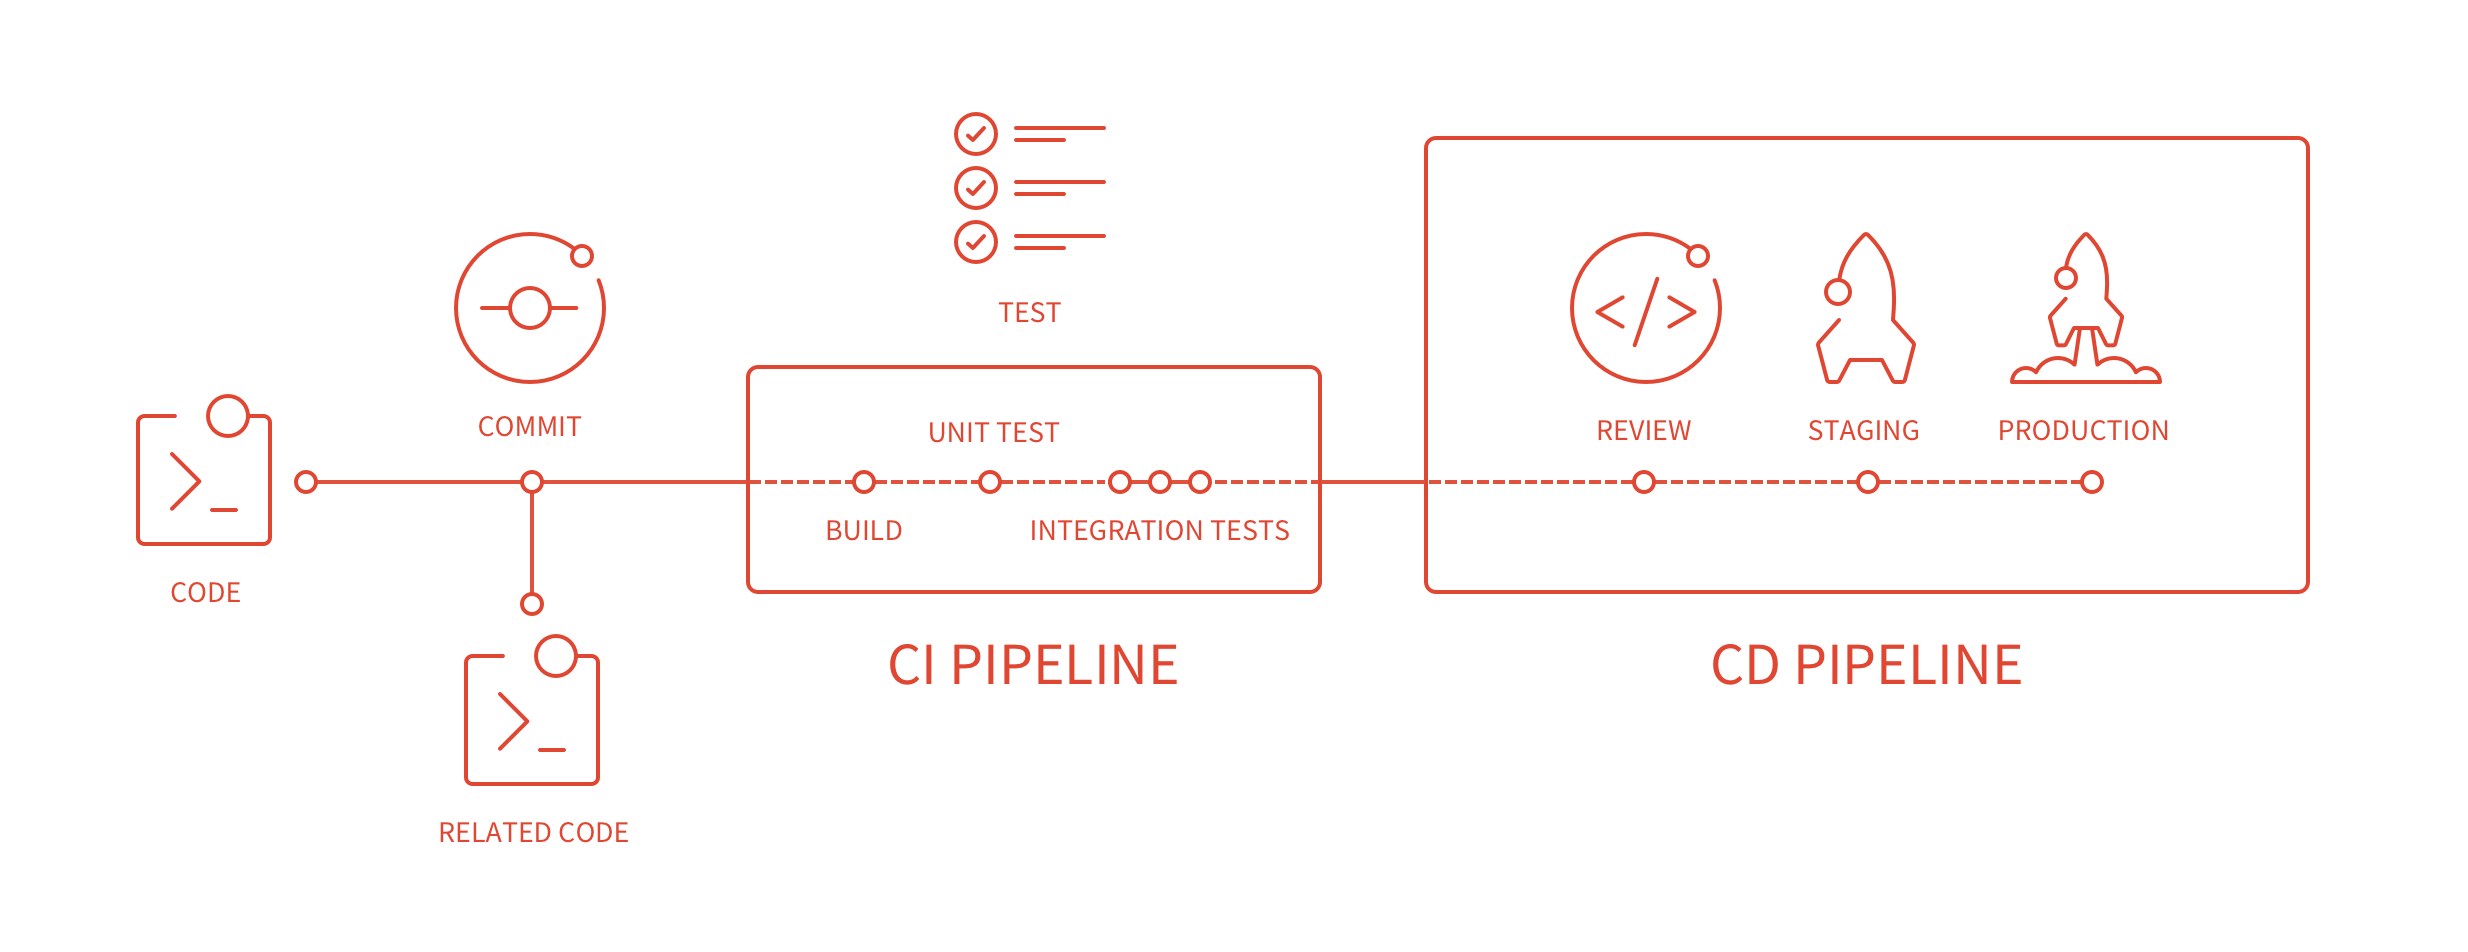
\includegraphics[scale=0.18]{./images/cicd_pipeline_gitlab.png}
		\caption{Rappresentazione del processo di CI/CD presso GitLab. Immagine dal sito web del produttore: \url{https://docs.gitlab.com/ee/ci/}}
	\end{center}
\end{figure}

\begin{figure}[H]
	\begin{center}
		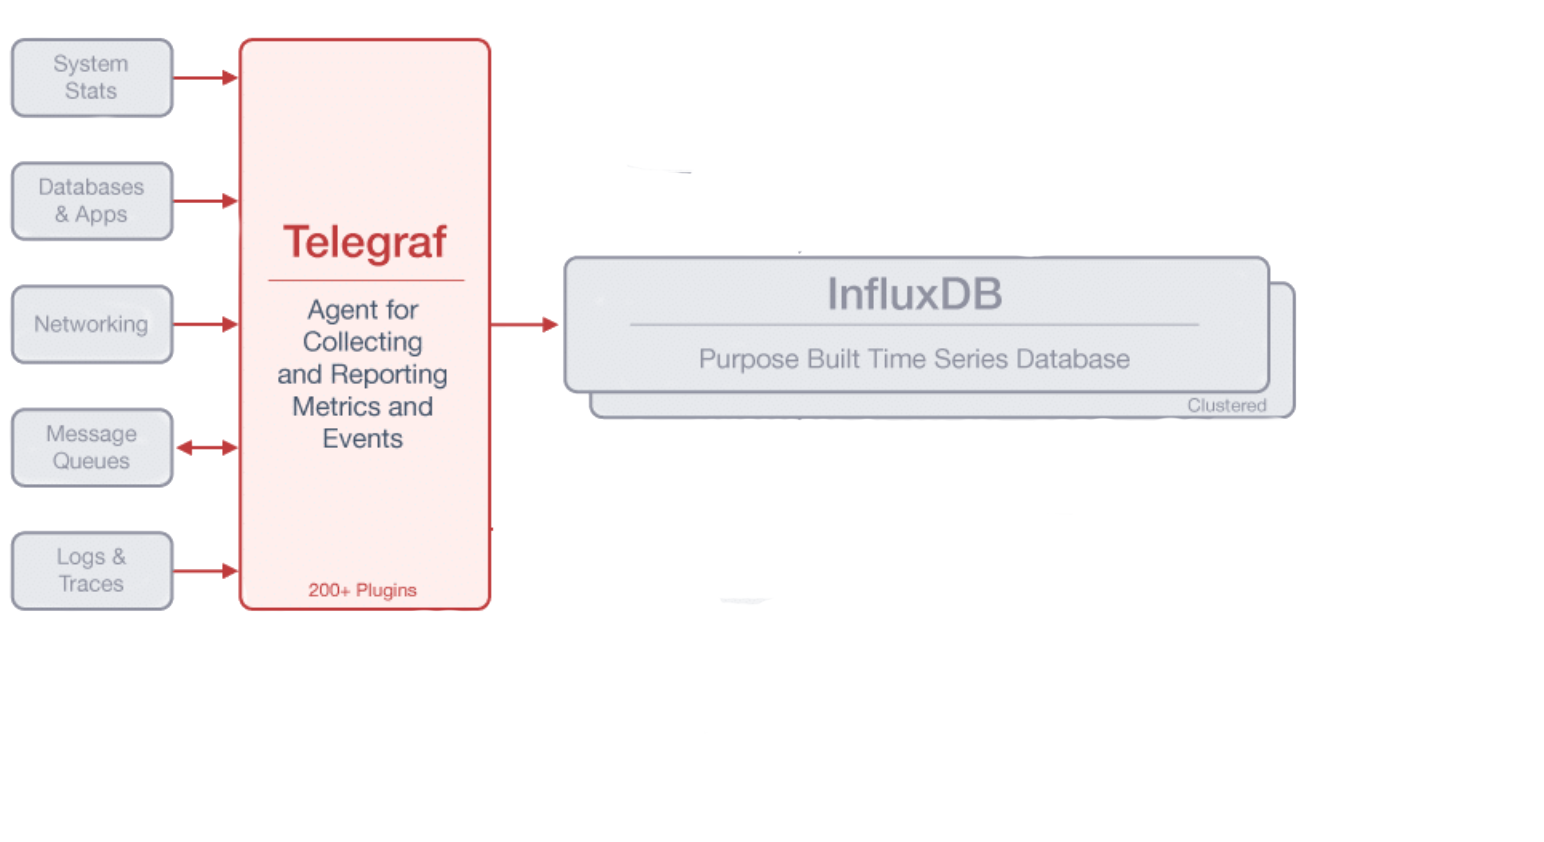
\includegraphics[scale=0.4]{./images/influxTelegraf.png}
		\caption{Rappresentazione del funzionamento di Telegraf e InfluxDB. Immagine dal sito web del produttore: \url{https://www.influxdata.com/time-series-platform/telegraf}}
	\end{center}
\end{figure}

\paragraph{Integrazione}\label{Progettazione_Integrazione}\-\\
L'attività di integrazione sarà effettuata utilizzando il servizio disponibile su \textit{GitLab}, piattaforma per repository utilizzata dal gruppo per il versionamento dei file sorgente.\\
Questo servizio implementa un modello di integrazione continua: ad ogni commit\glossario nel repository\glossario, \textit{GitLab} creerà automaticamente la build ed andrà ad eseguire i test di unità. In questo modo è possibile rilevare tempestivamente eventuali errori.\\
Per quanto riguarda il code coverage\glossario si utilizzerà un servizio messo a disposizione da \textit{GitLab}.\\

\paragraph{Diagrammi}\label{Progettazione_Diagrammi}\-\\
Per rendere più chiare le scelte progettuali adottate, si farà largo uso di diagrammi UML 2.0\glossario. Essi potranno essere di diversi tipi:
\begin{itemize}
	\item \textbf{Diagrammi dei Casi d'Uso}: dedicati alle funzionalità offerte dal sistema;
	\item \textbf{Diagrammi delle Classi}: dedicati alla descrizione degli oggetti che fanno parte del sistema, e le loro dipendenze;
	\item \textbf{Diagrammi dei Package}: dedicati alla descrizione delle dipendenze tra gli oggetti raggruppati in un package;
	\item \textbf{Diagrammi di Sequenza}: dedicati alla descrizione della collaborazione nel tempo tra un gruppo di oggetti;
	\item \textbf{Diagrammi di Attività}: dedicati ala descrizione della logica procedurale.
\end{itemize}

\paragraph{Obiettivi della Progettazione} \-\\
\label{Progettazione_Obiettivi}
La Progettazione serve per garantire che il prodotto sviluppato soddisfi le proprietà ed i requisiti delineati durante l'attività di analisi, ponendosi come obiettivi:
\begin{itemize}
	\item Garantire la qualità di prodotto sviluppato, perseguendo la correttezza percostruzione;
	\item Rendere chiara e comprensibile l'architettura progettata per gli stakeholder;
	\item Mantenere bassa la dipendenza tra le varie parti del prodotto favorendo la modularità ed il riuso;
	\item Ottimizzare l'uso delle risorse.
\end{itemize}